%%%%%%%%%%%%%%%%%%%%%%%%%%%%%%%%%%%%%%%%%%%%%%%%%%%%%%%%%%%%%%%%%%%%%%%%%%%%%%%%
% simulation.tex: Chapter on MC production: Here Mostly ECAL Timing
%%%%%%%%%%%%%%%%%%%%%%%%%%%%%%%%%%%%%%%%%%%%%%%%%%%%%%%%%%%%%%%%%%%%%%%%%%%%%%%%
\chapter{ECAL Time Reconstruction and Calibration}
%%%%%%%%%%%%%%%%%%%%%%%%%%%%%%%%%%%%%%%%%%%%%%%%%%%%%%%%%%%%%%%%%%%%%%%%%%%%%%%%
The time of an electromagnetic object such as a photon is extracted at the level of individual crystals called reconstructed hits~(rechits). The recorded time of the photon is the crystal calibrated time where the Time-Of-Flight~(TOF) as well as the time to transmit the recorded signal from the front-end detectors to the back-end readout electronics is removed such that on average the time is zero for a photon produced at the nominal proton-proton collision point and travelling at speed of light and then impinges at the surface of the crystal.  There are separate algorithms for extracting and calibrating the crystals using the rechit time. This calibrated time is considered the reconstructed time~($T_{RECO}$). 
Measuring the difference in timing between any two reconstructed objects ( individual crystals or electromagnetic objects) originating from the same nominal point and thus assumed in principle to have the same time give the timing resolution of the detector as well as the crystal-to-crystal synchronization factor.  $T_{RECO}$ of a photon can be defined in either of the following ways:
\begin{enumerate}
\item Seed Time: The time of the highest energy crystal or rechit in the highest energy basic cluster of the photon supercluster denoted as $T_{SEED}$
\item The Mean Time: This is the error weighted mean time of all the crystals in the photon supercluster denoted as $T_{CLUSTER}$ or $T_{MEAN}$ and is defined as follows:
\begin{equation}
T_{CLUSTER} = T_{MEAN} = \frac{\sum_{i=1}^N\frac{T_{i}}{\sigma_{i}^{2}}}{\sum_{i=1}^{N}\frac{1}{\sigma_{i}^{2}}} 
\end{equation}
\newline
 where N is the number of crystals in seed basic cluster of photon supercluster. 

\end{enumerate}
\subsection{Electromagnetic Calorimeter Readout Chain}
%%%%%%%%%%%%%%%%%%%%%%%%%%%%%%%%%%%%%%%%%%%%%%%%%%%%%%%
The readout system of the CMS ECAL better described in \cite{ECALREADOUT}, consists of an on-detector Very Front-End ~(VFE) part and a digital readout and processing part or off-detector placed in a counting room. The on-detector part and the off-detector parts communicated through a large number of optical links. A simple picture of the readout chain is shown in fig{FIXME:Fig readout Chain}.

%%%%%%%%%%%%%%%%%%%%%%%%%%%%%%%%%%%%%%%%%%

%%%%%%%%%%%%%%%%%%%%%%%%%%%%%%%%%%%%%%%%%%%%%%%%%%%%%%%%%%%%%%%%%%%%%%%%%%%%%%%%
\subsection{Timing Extraction}
%%%%%%%%%%%%%%%%%%%%%%%%%%%%%%%%%%%%%%%%%%%%%%%%%
The digital  filtering~(DF) technique is used to reconstruct the amplitude collected by the \pb crystals.

%%%%%%%%%%%%%%%%%%%%%%%%%%%%%%%%%%%%%%%%%%%%%%%%%
\subsection{Calibration Procedure}
%%%%%%%%%%%%%%%%%%%%%%%%%%%%%%%%%%%%%%%%%%%%%%%%%%%%%
The Ecal time is calibrated such that the the time travel by a photon or any highly relativistic  particle  produce at the nominal region of CMS proton-proton collision is on average 0 ns. This ensures that if a particle in detected with a significantly large positive time, then it is either this particle is travelling with a very small velocity (slowly moving particles or small $\beta << 1$ particle or it was produced as the decay product of stopped particle in the detector or it is a particle which is not travelling in a straight line but rather on a curved path to reach the ECAL.
%%%%%%%%%%%%%%%%%%%%%%%%%%%%%%%%%%%%%%%%%%%%%%%%%%%%
\subsection{ECAL Time Performance}
%%%%%%%%%%%%%%%%%%%%%%%%%%%%%%%%%%%%%%%%%%%%%%%%%%%%%%%%%%%%%%%%%%
The time performance of the ECAL crystals is studied and validated using events with a Z decay  i.e $\PZ \rightarrow \Pelectron \Ppositron$. 
\newline
The main idea is to use two reconstructed "objects" which in principle should have the same time and then use their time difference as a measure of the timing performance. We:
\begin{enumerate}
\item use two crystals within the same electron super cluster.
\item use the two electrons from the $\PZ$ decay. 
\end{enumerate}
In using electron super clusters, we considered following additional contributions to the electron time:
\begin{enumerate}
\item The bending of the electron path due to the presence of the 3.8~T magnetic field of the CMS detector.
\item  Displaced collisions  because "partons"~(subparticles) in the protons of the proton-proton~(p-p) bunches did not collide at exactly the collision point or Nominal Interaction point~(IP).
\item The collision developed over the full duration of the overlap of the proton bunches.
\end{enumerate}

The Time-Of-Flight~(TOF) of the electron from the IP is considered in the time calibration algorithm of the ECAL crystals.
Indeed, one assumption of using photons to time calibrate the ECAL crystals in that, they travel with the speed of light and so on average the time taken for a photon to travel from the IP until it impinges on the crystal surface in on average 0. With this assumption true only for Nominal Collisions i.e collisions originating for the IP and travelling straight to the ECAL crystals.
\newline


\begin{center}
\centering
\mbox{
\includegraphics[width=3in]{/home/tensr/Documents/ECAL_NOTES/PLOTS/2013/ECALTDRPLOTS/EB-EB-Time-of-seed.png}\quad
\includegraphics[width=3in]{/home/tensr/Documents/ECAL_NOTES/PLOTS/2013/ECALTDRPLOTS/EE-EE-Time-of-Seed.png}}
\captionof{figure}{Ecal absolute time of a single reconstructed electron in $\PZ \rightarrow \Pelectron \Ppositron$ decay. The electron time is the seed~(crystal with highest energy deposit)time of the electron.(a) in in EB and (b) in EE} 
\label{fig:ZeeTimePerformance}
\end{center}

%    \centering
%    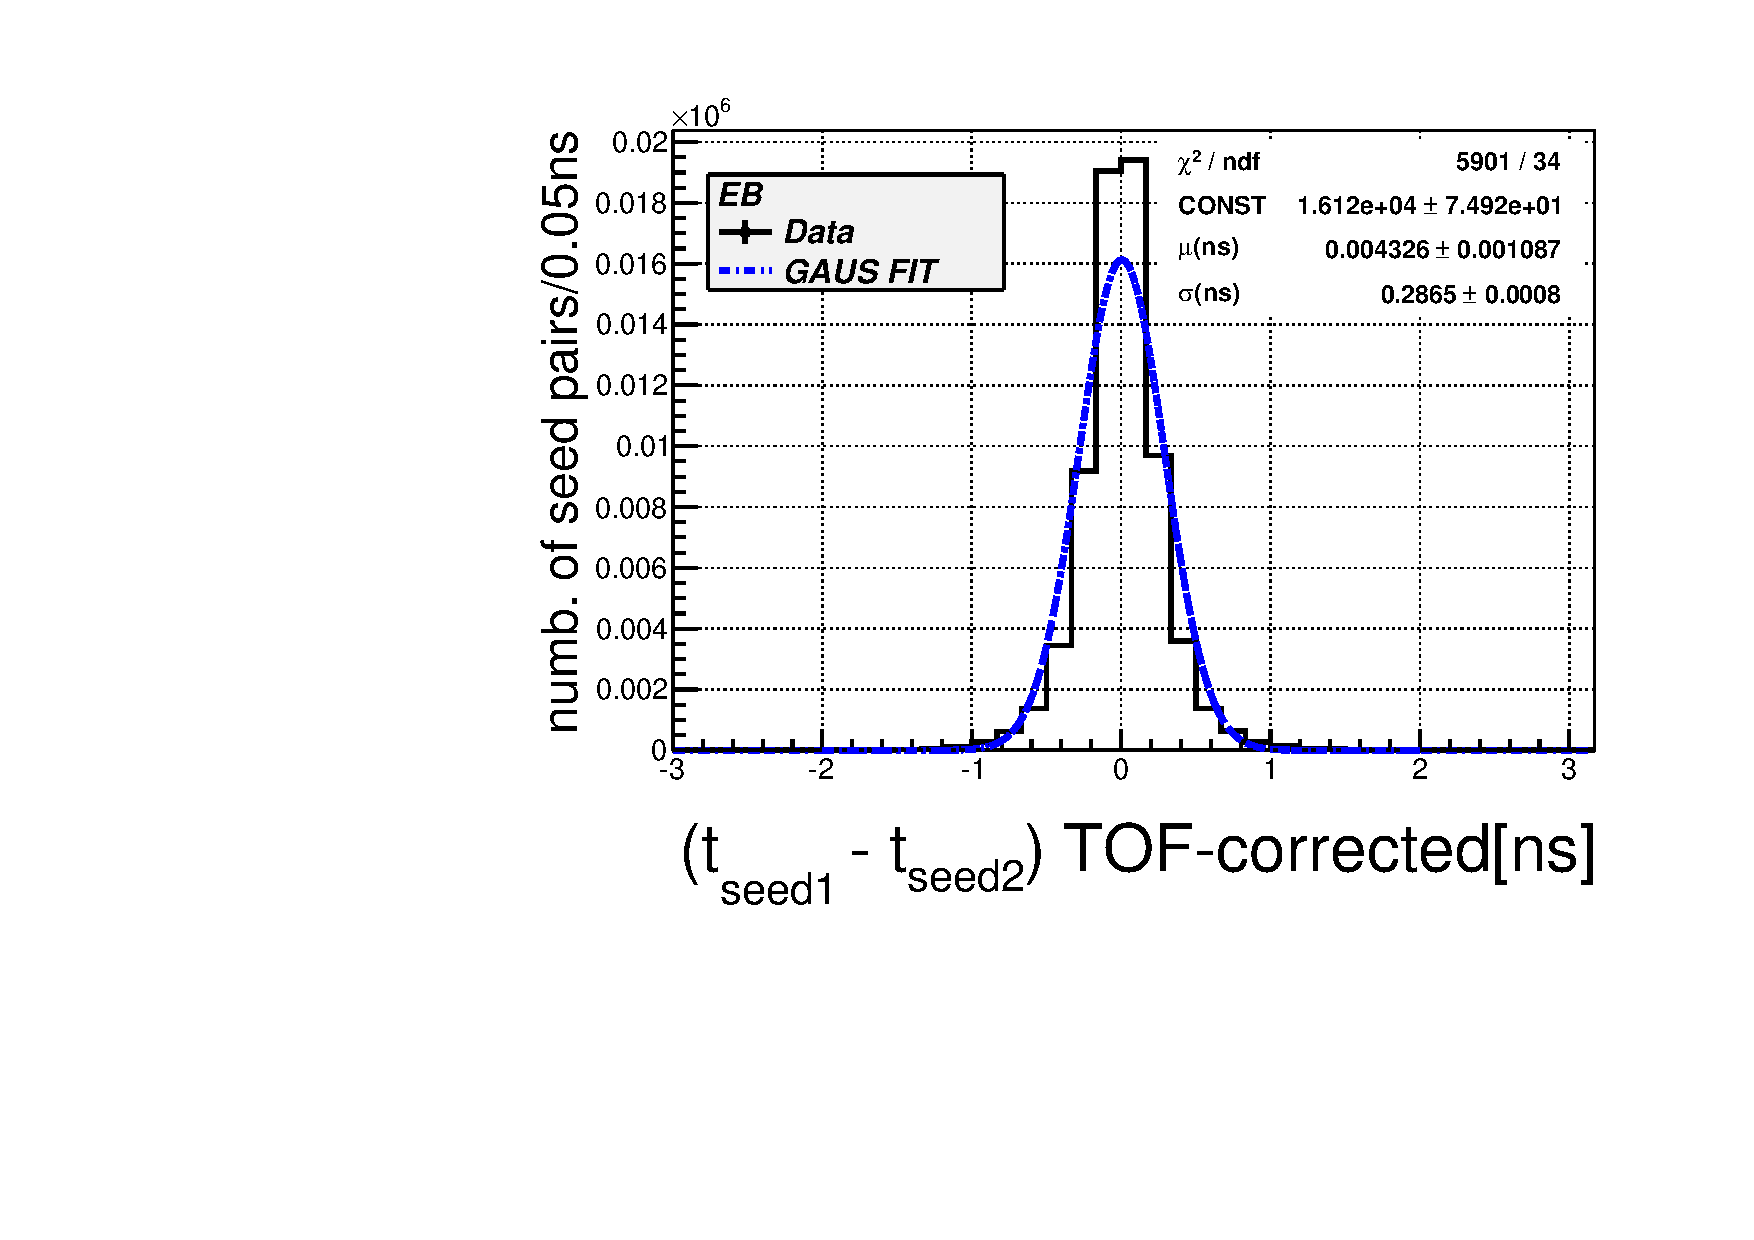
\includegraphics[width=0.8\textwidth]{/home/tensr/Dropbox/PHD_Thesis_HEP/PHD_THESIS/PHD/THESISPLOTS/EB-EB-TOF-Corr-difference-of-seed-Time-DoubleElectron_Run2012A.pdf}
%    \label{fig:awesome_image}


%\centering
%\begin{figure}[ht]       
%        \begin{subfigure}[a]{0.5\textwidth}
%        \centering
%        \includegraphics[width=0.4\textwidth{/home/tensr/Dropbox/PHD_Thesis_HEP/PHD_THESIS/PHD/THESISPLOTS/TOF-Corrected-Seed_Time_DoubleElectron_Run2012A-EB-EB.png}\caption{EB: TOF-Corrected Seed Time Difference}
%        \label{fig:EB TOF-Corr}
%        \end{subfigure}%
%        ~ %add desired spacing between images, e. g. ~, \quad, \qquad etc.
%         %(or a blank line to force the subfigure onto a new line)       
%        \begin{subfigure}[b]{0.5\textwidth}
%        \centering
%        \includegraphics[width=0.4\textwidth{/home/tensr/Dropbox/PHD_Thesis_HEP/PHD_THESIS/PHD/THESISPLOTS/TOF-Corrected-Seed_Time_difference_DoubleElectron_Run2012A-EE-EE.png}\caption{EE: TOF_Corrected Seed Time Difference}
%        \label{fig:EE TOF-Corr}
%        \end{subfigure}
%   \caption{Ecal time difference between the two reconstructed electrons in $\PZ \rightarrow \Pelectron \Ppositron$ decay. The electron time is the seed~(crystal with highest energy deposit) time with additional correction due to the time of flight of the electron.(a) in in EB and (b) in EE.}
%   \label{fig:ZeeTimePerformance}
%\end{figure}
%\begin{figure}[hbtp]
\begin{center}
\centering
\mbox{
\includegraphics[width=3in]{/home/tensr/Documents/ECAL_NOTES/PLOTS/2013/ECALTDRPLOTS/EB-EB-TOF-Corr-difference-of-seed.png}\quad
\includegraphics[width=3in]{/home/tensr/Documents/ECAL_NOTES/PLOTS/2013/ECALTDRPLOTS/EE-EE-TOF-Corr-difference-of-seed.png}}
\captionof{figure}{Ecal time difference between the two reconstructed electrons in $\PZ \rightarrow \Pelectron \Ppositron$ decay. The electron time is the seed~(crystal with highest energy deposit) time with additional correction due to the time of flight of the electron.(a) in in EB and (b) in EE} 
\label{fig:ZeeTimePerformance}
\end{center}
%\end{figure}

\begin{center}
 
  \begin{tabular}{|c|c|c|c|c|c|}
  % etc.
  \end{tabular}
 \captionof{table}{Table Comparing Timing Resolution performance of 2011 Vs 2012}
   \label{table1} % for use in \ref{table1} if you want to refer to the table number
\end{center}

%%%%%%%%%%%%%%%%%%%%%%%%%%%%%%%%%%%%%%%%%%%%%%
\label{ECAL Timing Calibration_chapter}
